% Search baseline solve rate by coupling, at fixed fold depth.
% Generated by workspace/figures/make_coupling_solve_figure.mjs
% Sources: /Users/luxian/FoldOriganmi/workspace/RESULTS/cp-distance/attempts.jsonl; coupling from meta.json under /Users/luxian/FoldOriganmi/workspace/corpus/out/release
% Per SAMPLE, not per attempt. Split at coupling 4.
% depth 8: low 13/13, high 11/16
% depth 9: low 8/10, high 5/20
% depth 10: low 4/6, high 2/15
% model arm at the same split, drawn nowhere because the direction flips and the cells are tiny:
%   luna depth 8: low 2/11, high 0/9
%   luna depth 9: low 0/7, high 0/10
%   luna depth 10: low 0/4, high 1/11
%
% Standalone: pdflatex coupling_solve.tex
% In a paper: keep the tikzpicture, drop the documentclass wrapper.
\documentclass[border=2pt]{standalone}
\usepackage{pgfplots}
\pgfplotsset{compat=1.18}
\definecolor{vizA}{HTML}{2A78D6}
\definecolor{vizB}{HTML}{EB6834}
\begin{document}
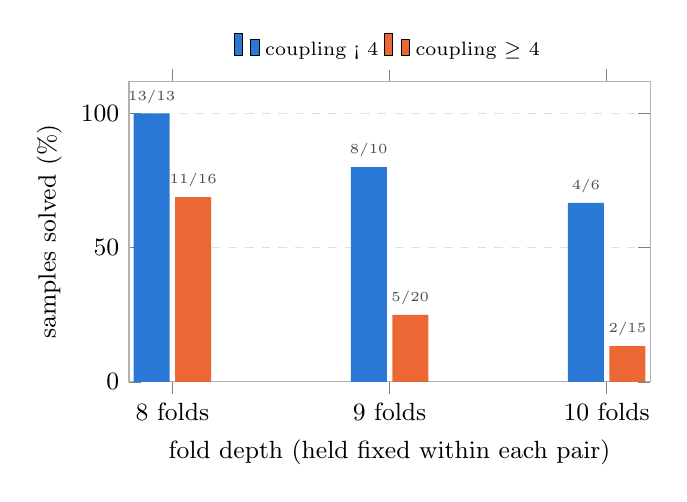
\begin{tikzpicture}
\begin{axis}[
  width=8.2cm, height=5.4cm,
  ybar, bar width=13pt,
  ymin=0, ymax=112,
  ylabel={samples solved (\%)},
  xlabel={fold depth (held fixed within each pair)},
  symbolic x coords={8 folds,9 folds,10 folds},
  xtick=data,
  point meta=explicit symbolic,
  nodes near coords={\pgfplotspointmeta},
  every node near coord/.append style={font=\tiny, color=black!70},
  tick label style={font=\small},
  label style={font=\small},
  legend style={font=\scriptsize, at={(0.5,1.18)}, anchor=north, legend columns=-1, draw=none},
  ymajorgrids, grid style={gray!25, dashed},
  axis line style={gray!60},
]
\addplot[fill=vizA, draw=none] coordinates {(8 folds,100.0) [13/13] (9 folds,80.0) [8/10] (10 folds,66.7) [4/6]};
\addlegendentry{coupling < 4}
\addplot[fill=vizB, draw=none] coordinates {(8 folds,68.8) [11/16] (9 folds,25.0) [5/20] (10 folds,13.3) [2/15]};
\addlegendentry{coupling $\geq$ 4}
\end{axis}
\end{tikzpicture}
\end{document}
